\chapter{Introduction to Fluid-Structure Interaction}
Fluid-Structure Interaction(FSI) can be observed all around us in nature. From a flag waving in the wind to a large windmill at sea. 
When we breath in air and our lungs expand. When our hearts fill up with blood and muscles contract to push the blood into our veins. These are all examples of fluids and structures interacting. A flag waving in the wind is mainly air(fluid) exerting force on the flag which is thin and usually made of light fabric. The fluid makes the flag flutter. The solid can also move the fluid. When we push our fingers into a water balloon. We deform the structure around the fluid, exerting force on the fluid. \newline

A scary example of FSI is the collapse of the Tacoma Narrows Bridge in 1940 \cite{Billah1991}. The bridge collapsed only two months after being opened. The collapse was due to strong winds(64 km/h) interacting with the bridge, making it flutter and ultimately collapse. No human life was lost in the collapse, but a Cocker Spaniel name Tubby left in a car was not so lucky. \newline

Another example of FSI are inter-cranial aneurysms, which are balloon shaped geometries often occurring in a bifurcation(where a blood vessel splits into two vessels), due to weak vessel walls. Bursting of one of these aneurysms in the skull can have fatale consequences. The need to model FSI is crucial to understand these problems. \newline
\begin{figure}
\centering
\begin{minipage}{.51\textwidth}
  \centering
  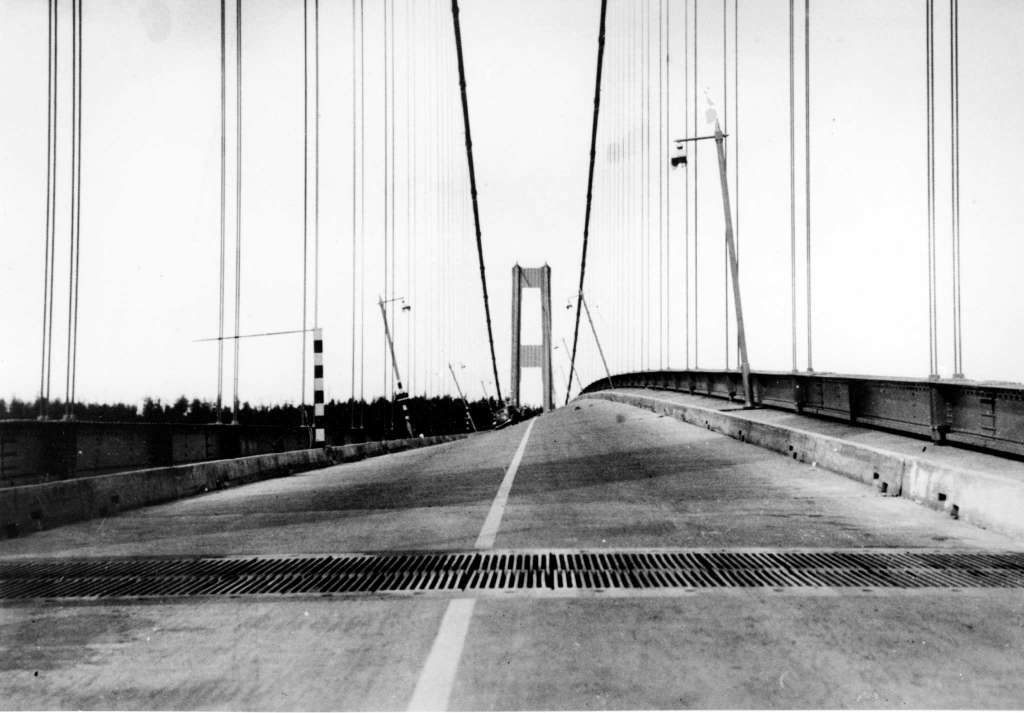
\includegraphics[width=.95\linewidth]{./IntroductionToFSI/tacoma2.jpeg}
  \caption{Tacoma bridge still standing with large deformations}
  \label{fig:test1}
\end{minipage}%
\begin{minipage}{.50\textwidth}
  \centering
  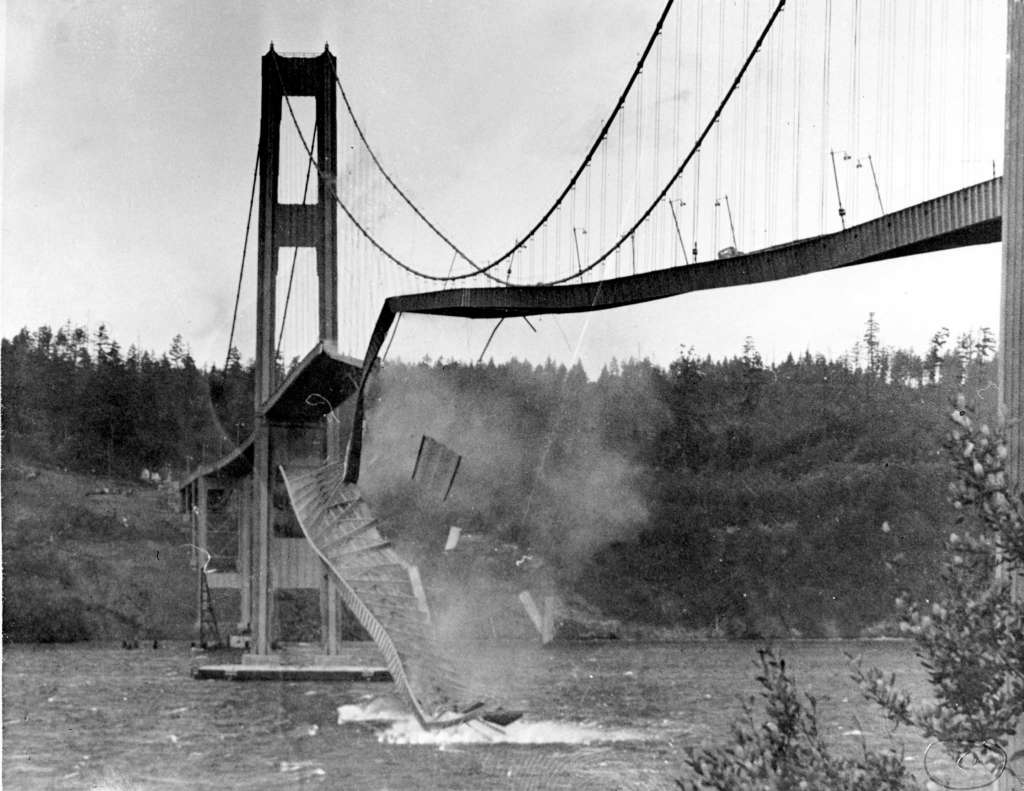
\includegraphics[width=.95\linewidth]{./IntroductionToFSI/tacoma3.jpeg}
  \caption{Tacoma bridge collapsed}
  \label{fig:test2}
\end{minipage}
\end{figure}

Modelling fluid dynamics is called \textit{Computational Fluid Dynamics} (CFD). I would argue the same for FSI. That we call modeling FSI for \textit{Computational Fluid Structure Interaction} (CFSI)
Modeling FSI is used today when constructing for instance windmills. These windmills are usually rigid, hence giving a big difference in density between fluid and structure. The structure will in this case only give rise to small deformations. However modeling FSI in hemodynamics(dynamics of blood flow) deems more challenging. In these cases the densities in fluid and solid are much more similar and usually inducing large deformations. Also in both of these cases the fluid flow tends to transition to turbulence. We can see that these challenges gives the need to have rigid stabile FSI solvers, solvers which can handle large deformations and high fluid velocity. \newline

Tthe main goal of this master thesis is to build a framework to solve the FSI problem, investigating different approaches and schemes. The framework will be validated and verified using the \textit{Method of Manufactured Solutions}, accompanying a wide range of benchmarks.  



\begin{comment}
Fluid-Structure Interaction problem can be observed all around us in nature, from large industrial engineering complexes to the smallest blood vessels in the human body. A large scale example is the collapse of the Tacoma Narrows Bridge that collapsed in 1940 only two months after being opened. The collapse was due to aero-elastic fluttering from strong winds. No human life was lost in the collapse, but a cocker spaniel name Tubby left in a car was not so lucky. The construction of windmills are a second example of the Fluid-Structure Interaction problem. Todays windmills are rigid and hence giving a big difference in density between fluid and structure, $ \rho_s >> \rho_f $. The structure will therefore only give rise to small deformations. However applying FSI to hemodynamics( dynamics of blood flow ) deems more challenging. One FSI hemodynamic problem are inter-cranial aneurysms, which are balloon shaped geometries often occurring where a blood vessel splits into two parts, due to weak vessel walls. Bursting of one of these aneurysms in the skull can have fatale consequences. With fluid and structure densities more equal than the previous example, the structure has an elastic character giving under the right circumstances large deformations. The blood flow also transitions to turbulent flow. This combination gives the need for a rigid stabile solver. Therefore the main goal of this master thesis is to build a framework to solve the FSI problem, investigating different approaches and schemes. The framework will be validated and verified using MMS, companying a wide range of benchmarks.  
\end{comment}

